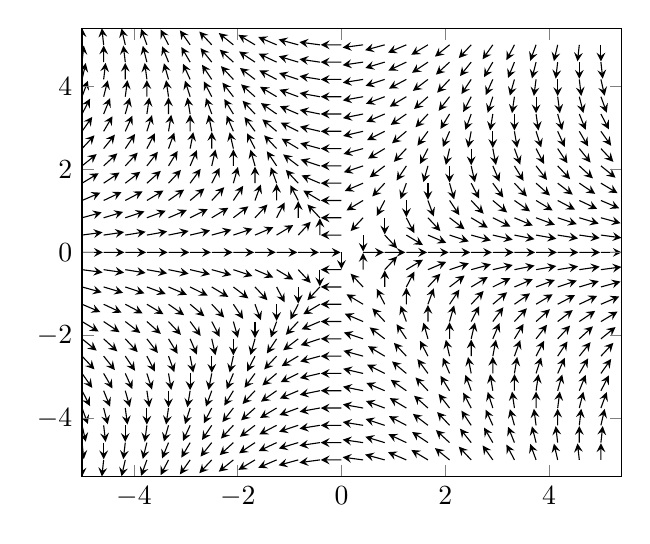
\begin{tikzpicture}
\begin{axis}[
view = {0}{90},
%unbounded coords=jump,
   % x filter/.expression={
   %     x>9 ? nan : x
   % },
%unbounded coords=jump,
  %  y filter/.expression={
   %     y>9 ? nan : y
  %  }
]
\addplot3[
        quiver = {
                u = {(x^2-y^2)/sqrt((x^2-y^2)^2+(2*x*y)^2)},
                v = -{(2*x*y)/sqrt((x^2-y^2)^2+(2*x*y)^2)},
            scale arrows = 0.4},
            domain = -5:5,
            domain y = -5:5,
        -stealth] {0};
\end{axis}
\end{tikzpicture}
\caption*{Representación vectorial normalizada}